\documentclass[12pt]{article}

%%%%%%%%%%%%%%%%%%%%%%%%%%%%%%%%%%%%%%%%%%%%%%%%%%%%%%%
\usepackage[margin=1.65cm]{geometry}
\usepackage{blindtext}
\usepackage[utf8]{inputenc}
\usepackage{graphicx}
\usepackage{titling}
\usepackage{changepage}
\usepackage[export]{adjustbox}
\usepackage{hyperref}
\usepackage[ngerman]{babel}
\title{\Huge Pflichtenheft für Projekt Dashboard}
\author{Michél Fischer, Eike Schaubeck, Lydia Kaiser, Michael Bendel}
\begin{document}
\maketitle
\tableofcontents
\newpage
%%%%%%%%%%%%%%%%%%%%%%%%%%%%%%%%%%%%%%%%%%%%%%%%%%%%%%%
\section{Einleitung}
Folgende Projektarbeit haben Eike Schaubeck, Michael Bendel, Michel Fischer und Lydia Kaiser zusammen erarbeitet, wobei André Bauer als Betreuer fungierte.\\
Die Idee von diesem Projekt ist, ein Dashboard in einer Web-Anwendung zu programmieren, um die Planung mittels Kalender einfacher, strukturierter und übersichtlicher zu gestalten. Es soll ein Überblick über das Wetter, die Bus/Bahnverbindungen und weitere wichtige Termine geschaffen werden, sodass man nicht mehr zwischen mehreren Apps wechseln muss. Die Oberfläche des Programms soll ansprechend und intuitiv gestaltet werden. Um unnötigen Datenverbrauch zu vermeiden, soll das Dashboard asynchron geupdatet werden. 
\section{Kriterien}
%%%%%%%%%%%%%%%%%%%%%%%%%%%%%%%%%%%%%%%%%%%%%%%%%%%%%%%
Folgende Kriterien wurden zur Eingrenzung der Funktionalitäten definiert:\\
Hierbei wird jeweils auf die Bereiche Datenbank, GUI und Controller eingegangen.
\subsection{Muss-kriterien}
\subsection*{Datenbank}
Der Nutzer kann Termine aus seinem Kalender verwalten. Dazu gehört das Laden, das Hinzufügen, das Löschen und das Ändern von Terminen.
\subsection*{GUI}
Die graphische Oberfläche soll das (aktuelle) Wetter, Bus/Bahnverbindungen und Termine in Textform anzeigen.
\subsection*{Controller}
\subsubsection*{$\bullet$\quad Bus/Bahnverbindung}
Passend zu den Terminen sollen Bus/Bahnverbindungen angezeigt werden. Die Verbindungen sollen mit Start-/Zielbahnhof und der jeweiligen Zeit angegeben werden. Wenn Umstiege vorhanden sind, dann sollen auch die Zwischenhaltestellen (ebenfalls mit Zeit) angezeigt werden.
\subsubsection*{$\bullet$\quad Wetter}
Es soll das aktuelle Wetter und eine Prognose von kleiner gleich vier Tagen zu sehen sein. Dabei soll der Standort, die Regenwahrscheinlichkeit, die aktuelle Temperatur,die Niederschlagsart sowie die Tiefst- und Höchsttemperatur dargestellt werden. Bei der Auswahl einer Bahnverbindung soll die Wetterlage am Start-/Zielort angezeigt werden.
\subsubsection*{$\bullet$\quad Kaledereinträge}
Kalendereinträge werden unterteilt in Termine und Notizen. Dabei kann man bei Terminen den Namen, Start- und Endzeit und den Ort angeben.\\
Die Notizen bestehen aus einem begrenzt langen String.
\subsubsection*{$\bullet$\quad Notizen}
Die Notizen werden als Text angezeigt.
\subsubsection*{$\bullet$\quad Allgemein}
Die Wetterdaten und die Verbindungsdaten sollen standortbezogen sein. Die Aktualisierung der einzelnen Elemente soll dabei asynchron durchgeführt werden.\\
Die Bedienung des Dashboards soll auch über die Kommandozeile möglich sein.\\
Beim Auftreten von Fehleren bei dem Verbindungsaufbau, nicht verwertbaren Angaben zu Zeit und Orten sollen passende Fehlermeldungen angezeigt werden.

%%%%%%%%%%%%%%%%%%%%%%%%%%%%%%%%%%%%%%%%%%%%%%%%%%%%%%%%
\subsection{Kann-kriterien}
\subsection*{GUI}
Die räumliche Anordnung der Elemente soll für den Nutzer frei wählbar sein, wobei auch Elemente ein- und ausgeblendet werden können.
\subsection*{Controller}
\subsubsection*{$\bullet$\quad Weitere Funktionen und Termine}
Der Nutzer hat die Möglichkeit eine direkte Notiz zu speichern. Außerdem können die Geburtstage im Kalender verwaltet werden und mit Namen und Alter angezeigt werden.
\subsubsection*{$\bullet$\quad Allgemein}
Die Synchronisationsrate kann vom Benutzer frei gewählt werden.
%%%%%%%%%%%%%%%%%%%%%%%%%%%%%%%%%%%%%%%%%%%%%%%%%%%%%%%%%
\subsection{Abgrenzungskriterien}
\subsection*{Datenbank}
Es können keine Datenanhänge im Kalender angelegt werden.
\subsection*{Controller}
\subsubsection*{$\bullet$\quad Wetter}
Weitere Daten zum Wetter könne nicht abgerufen werden und die Temperatur wird nur in Grad Celsius ausgegeben. Eine Prognose für mehr als vier Tage ist nicht möglich.
\subsubsection*{$\bullet$\quad Bus/Bahnverbindung}
Eine manuelle Abfrage von Bus/Bahnverbindungen ist nicht möglich. Nur auf den Termin bezogene Verbindungen stehen zur Verfügung.
\subsubsection*{$\bullet$\quad Termine}
Termine (als Datentyp String) können nicht beliebig lang sein.

\section{Technologien}
\subsection*{APIs für Dienste}
\begin{itemize}
\item{Für Wetter(prognose): DarkSky\\ \url{https://darksky.net/dev}}
\item{Für Bahnverbindungen: Google Directions API} \\ \url{https://developers.google.com/api-client-library/java}}
\end{itemize}
\subsection*{Konzepte}
\begin{itemize}
\item{AJAX;\quad \textit{Asynchronous JavaScript and XML}.}\\
\newline
Wie schon in den Muss-Kriterien genannt, sollen sich die einzelnen Module der Anwendung asynchron aktualisieren, wozu sich die Verwendung von AJAX anbietet.
\end{itemize}
\subsection*{Programmiersprachen}
\begin{itemize}
\item{HTML5 mit Bootstrap}
\item{JavaScript}
\item{Java 13 unter Benutzung von JSP's}

\end{itemize}

\newpage
\section{Diagramme}
\subsection*{UML-Klassendiagramm}
\begin{figure}[h]
	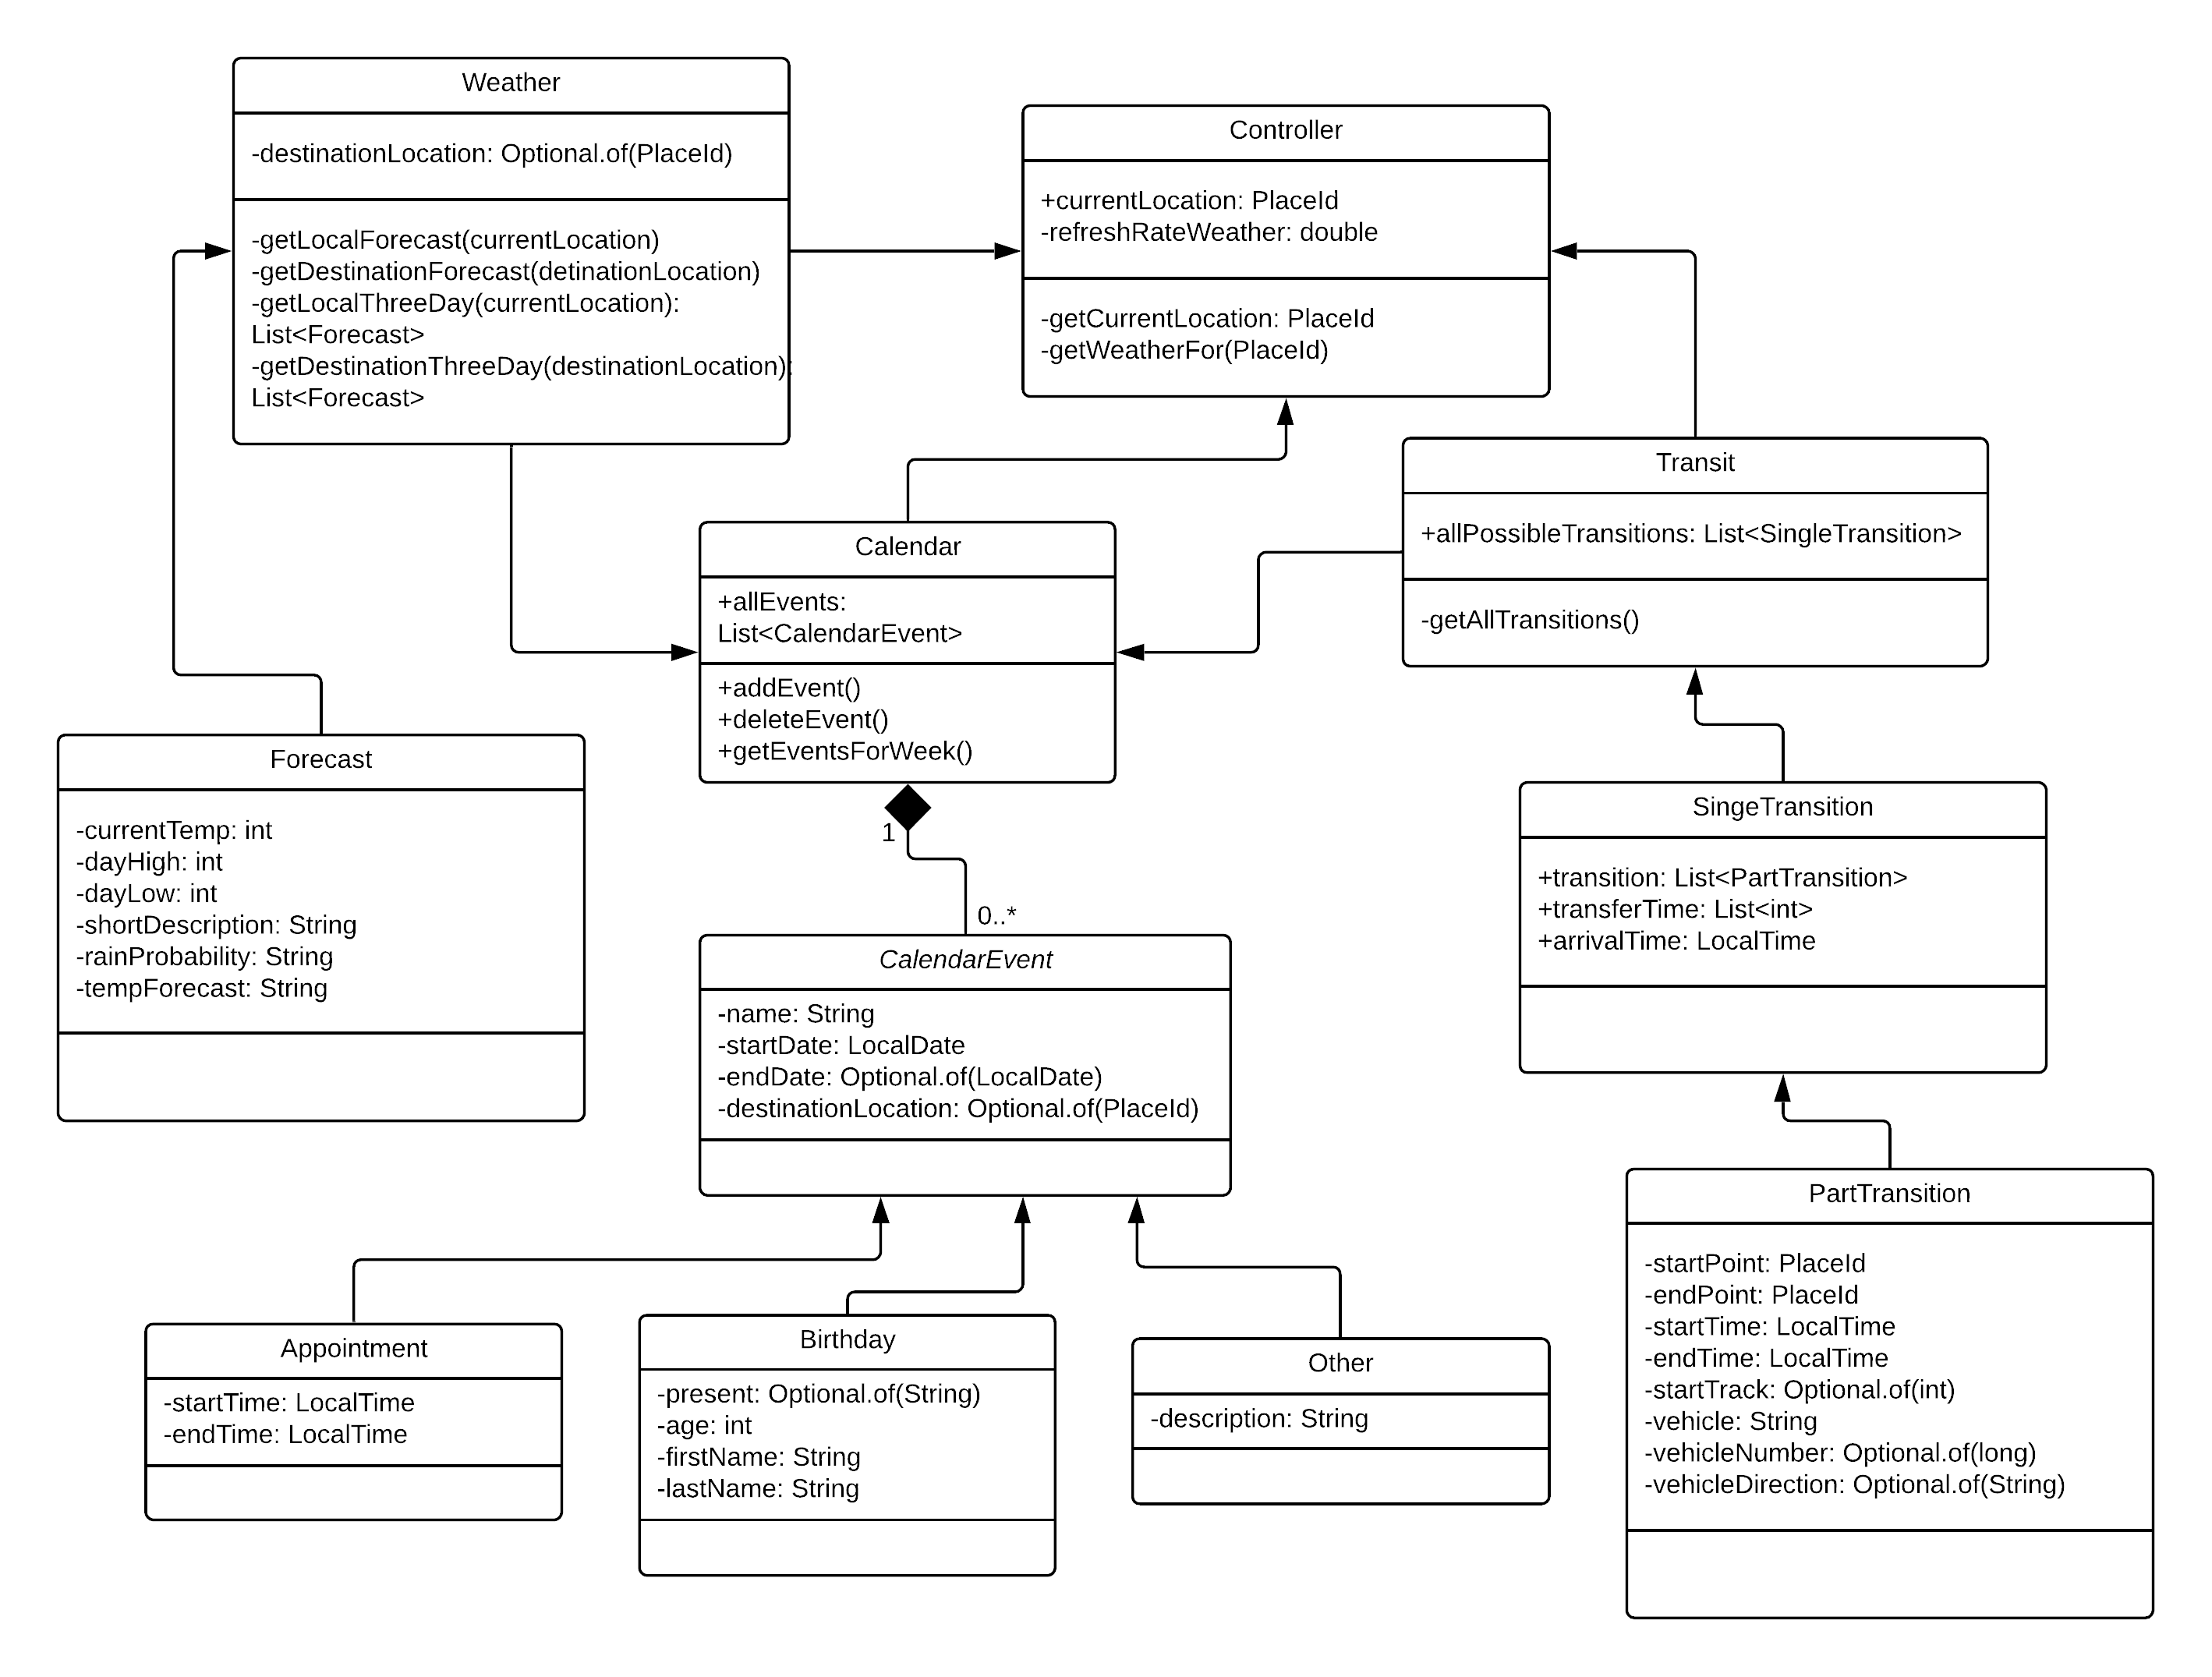
\includegraphics[width=1.1\textwidth,left]{CalendarUMLReformatted.png}
\end{figure}
\newpage
\section{Zeitplan}
Beim Planen des Projekts ergab sich der Zeitplan zur Realisierung wie folgt:\\
\newline
\begin{tabular}{|l|l|}
\hline
\textbf{Kalenderwoche} & \textbf{Fortschritt}\\
\hline
44 & Fehlerbehebung und Fertigstellung des Wettermoduls\\
\hline
45 & Einarbeiten in Bootstrap, Ajax und JSP's\\
\hline
46-47 & Erste Version von Kalender- und Bahnmodul\\
\hline
48 & Zusammenfügen aller Module und Bugfixing\\
\hline
49-50 & Erster GUI-Entwurf\\
\hline
51-52 & GUI-Fertigstellung und Bugfixing, ggf. sonstige Optimierungen\\
\hline
1-3  (2020) & Sämtliche Handbücher, Präsentation, etc.\\
\hline
4  (2020)& Testfälle und Endversion\\
\hline
\end{tabular}
\section{Einsatz}
\subsection*{Anwendungsbereich}
Das Dashboard soll einen Überblick über den kommenden Tag, oder auch die kommende Woche schaffen, wodurch die Planung und das Zeitmanagement des Alltags erleichtert werden soll. Der Nutzer kann auf einen Blick sehen, welche wichtigen Termine anstehen und somit seinen Tagesablauf anpassen.
\subsection*{Zielgruppe}
Die Anwendung richtet sich an Benutzer, die ihren Kalender als Terminplaner verwenden und somit die Möglichkeit haben, auf einfache Weise einen strukturierten Einblick über ihre Termine zu bekommen.
\end{document}
